


\section{Pirate Game}
\label{sec:pirate}

\begin{emph}
On selecting the problem...
\end{emph}


\subsection{Problem Description}
\label{subsec:description}

The original Pirate Game is a multi-player version of the Ultimatum game that was first published as a mathematical problem in the Scientific American as a mathematical problem posed by Omohundro\cite{Stewart1999}. The main objective of the Pirate Game was to present a fully explainable problem with a non-obvious solution. The problem can be formulated as it follows:

\begin{quotation}
Suppose there are 5 rational pirates: A; B; C; D; E. The pirates have a  loot of 100 indivisible gold coins to divide among themselves.


As the pirates have a strict hierarchy, in which pirate A is the captain and E has the lowest rank, the highest ranking pirate alive will propose a division. Then each pirate will cast a vote on whether or not to accept the proposal. 

If a majority or a tie is reached the goods will be allocated according to the proposal. Otherwise the proposer will be thrown overboard and the next pirate in the hierarchy assumes the place of the captain. 

We consider that each pirate privileges her survival, and then will want to maximize the number of coins received. When the result is indifferent the pirates prefer to throw another pirate overboard and thus climbing in the hierarchy. 
\end{quotation}

\subsection{Analysis}
\label{subsec:analysis_PG}

We can arrive at an equilibrium in this problem by using backward induction. At the end of the problem, supposing there are two pirates left, the equilibrium is very straight forward. As the highest ranking pirate can pass the proposal in spite of the other decision, her self-interest dictates that she will get the 100 gold coins. Knowing this, pirate E knows that any bribe other higher ranking pirate offers her will leave her better than if the game arrives to the last proposal. 

\begin{table}
\begin{center}
\begin{tabular}{cc}
  \num\putindeepbox[7pt]{\includegraphics[scale=0.20]{Pirates1/Slide1.PNG}}
    & \num\putindeepbox[7pt]{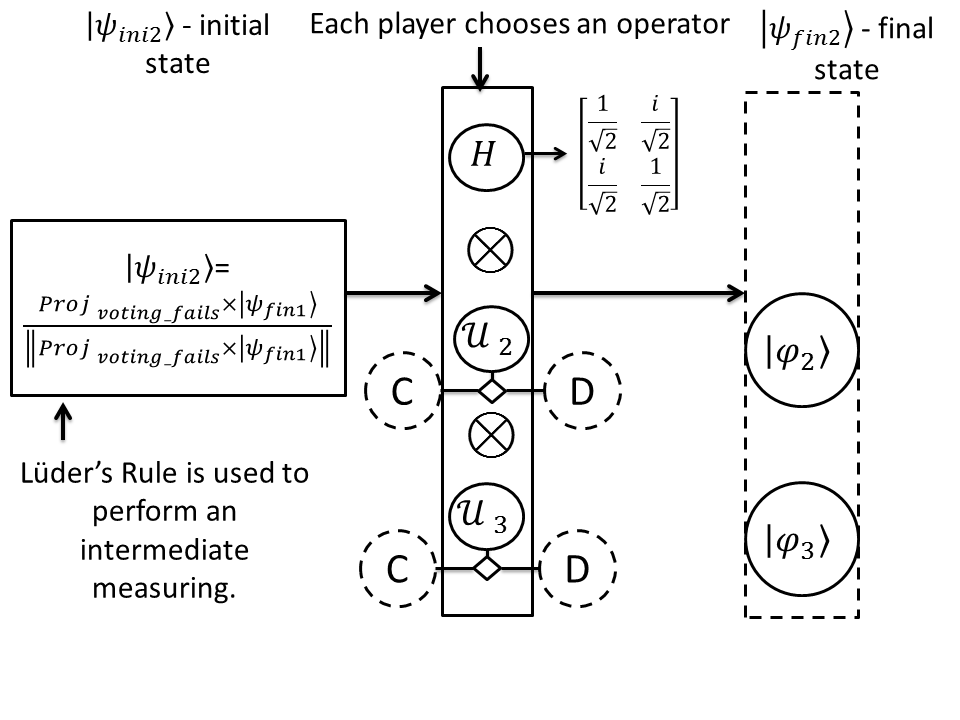
\includegraphics[scale=0.20]{Pirates1/Slide2.PNG}} \\
  \num\putindeepbox[7pt]{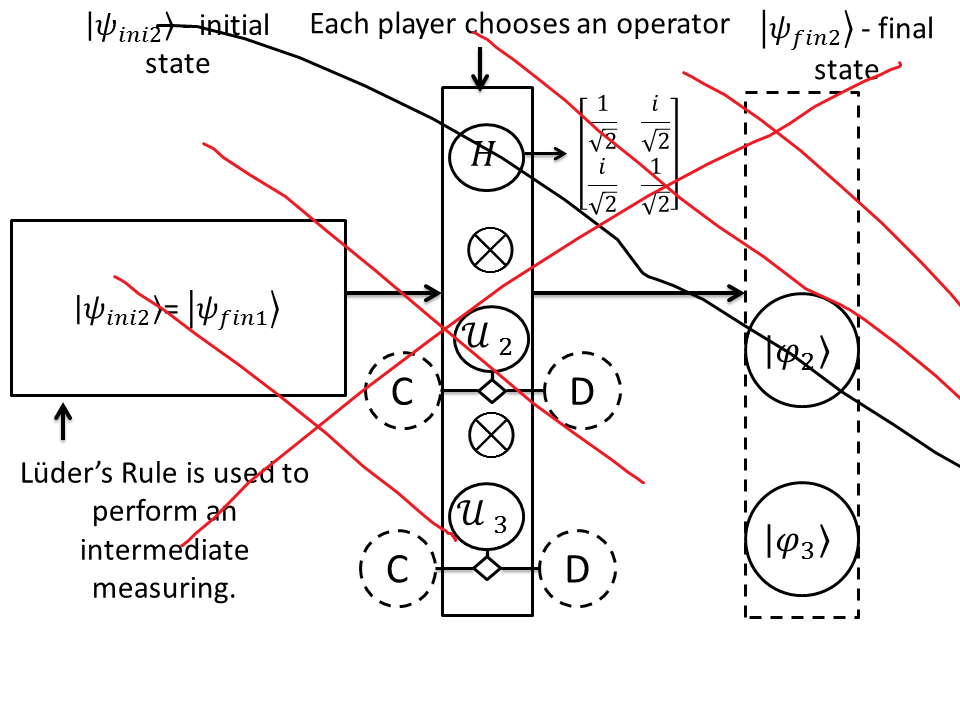
\includegraphics[scale=0.20]{Pirates1/Slide3.PNG}}
    & \num\putindeepbox[7pt]{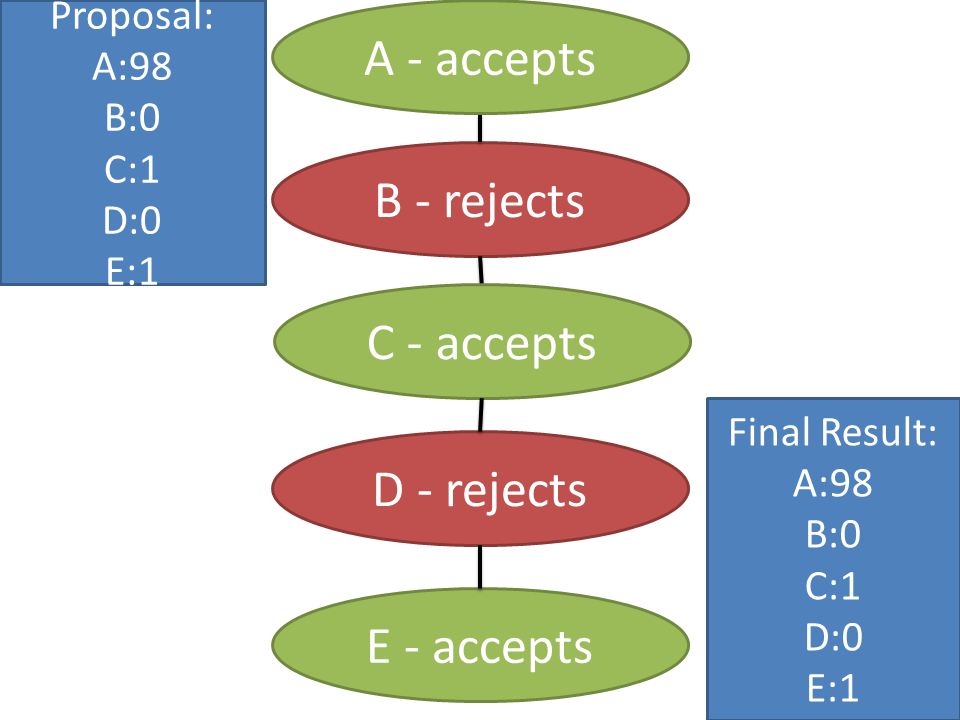
\includegraphics[scale=0.20]{Pirates1/Slide4.PNG}} \\
\end{tabular}
\caption{The equilibrium for the Pirate Game can be found through backward induction. From a), where there's only two pirates left, to d), that corresponds to the initial problem we define the best response.}
\label{tab:piratas_m}
\end{center}
 \end{table}

When applying this reasoning to the three pirate move, as pirate C knows she needs one more vote to pass her proposal and avoiding death, she will offer the minimum amount of coins that will make pirate E better off than if it comes to the last stage with two pirates. This means that pirate C will offer 1 gold coin to pirate E, and keep the remaining 99 coins. 

With 4 pirates, B would rather bribe pirate D with 1 gold coin, because E would rather like climb on the hierarchy and getting the same payoff. Finally, with 5 pirates the captain (A), will keep 98 gold coins and rely on pirate C and E to vote in favour of the proposal, by giving 1 gold coin each.

We can generalize this problem for $N$ pirates. If we assign a number to each pirate, where the captain is number 1 and the lower the number the higher the rank. If the number of coins is superior to the number of pirates, the equilibrium will have the captain (highest ranking pirate), giving a gold coin to each odd pirate, in case the number of players alive is odd, while keeping the rest to herself. When we have a even number of players the captain will assign a gold piece to each pirate with a even number, and the the remaining coins to herself.

\section{Quantum Pirate Game}
\label{sec:quantum_pirate}

\subsection{Hypothesis}
\label{subsec:qhipothesis}

The original Pirate Game is posed from the point of view of the captain. How should she allocate the treasure to the crew in order to maximize her payoff.
We can find the a equilibrium to the original Pirates Game and, while the solution may seem unexpected at first sight, it is fully described using backwards induction. 

When modelling this problem from a quantum theory perspective we are faced with some questions. The main difference from the original problem will rely on how the system is set up. Will the initial conditions provide different equilibria? Is there a condition where we are left with the classical problem? Is it possible for a captain, in a situation where we have more than two pirates left, to acquire all the coins?

We propose to study this problem for the $2$ and $3$ player games and trying to extrapolate for $N$ players. We will analyse the role of entanglement and superposition in the game system. Another aspect worth studying is the variation in the coin distribution on the payoff functions for the players.



\subsection{Quantum Model}
\label{subsec:description_2}

In order to model the problem we will start by defining it using the definition of quantum game ($\Gamma$), referred in \ref{eq:quantum_game_six_tuple}, Section \ref{sec:background_quantum_game_theory}\cite{Fra2011a}. 

We want to keep the problem as close to the original as possible in order to better compare the results. Thus we will analyse the game from the point of view of the captain. Will her best response change?

In terms of mechanics and steps, this problem could be described using $3$ players and later extended to any number $N$ of players. 

We begin by assigning an offset to each pirate (in order to identify her), as in the Section \label{subsec:description}. The captain is number $1$ and the lower the number the higher the rank. 


\subsubsection{Strategic Space}
\label{subsec:strategic_space}

Each player will be able to manipulate a qubit in the system, in this case $\vert\varphi_{1}\rangle,\:\vert\varphi_{2}\rangle,$ and $\vert\varphi_{3}\rangle$, with one of two operators shown in Equation \ref{eq:operators_piratas_quanticos}. 

An operator is an unitary $2\times2$ matrix that is used to manipulate a qubit in the system.
This restriction of the strategic space is relevant to keep the problem as close to the classical version as possible. The two operators will correspond to the action of voting ``Yes'' or to Cooperate, and voting ``No'', meaning that they will not accept the proposal.  

The cooperation operator will be represented by the Identity operator ($o_{i0}$, where i identifies the qubit uppon which player i will act). When assigned to a qubit this operator will leave it unchanged. 

The defection operator ($D$), will be represented by one of Pauli's Operators - the Bit-flip operator. This operator was chosen because it performs the classical operation NOT on a qubit.

\begin{equation}
\label{eq:operators_piratas_quanticos}
\mathcal{U}_{i} = \begin{cases}
C = o_{i0}=\left[\begin{array}{cc}
1 & 0\\
0 & 1
\end{array}\right]\\
D = o_{i1}=\left[\begin{array}{cc}
0 & 1\\
1 & 0
\end{array}\right]
\end{cases} , i \in \{ 1, 2, 3 \}
\end{equation}


\subsubsection{Initial State}
\label{subsec:pirates_initialstate}

A game $\Gamma$ can be viewed as a system composed by players. The initial system will be set up by defining an entanglement coefficient $\gamma$, that affect the way the three qubits (belonging to the three pirate players), are related \ref{eq:estado_inicial_pg}. The concept of entanglement is crucial to explain some phenomena in Quantum Mechanics (Section \ref{subsec:entanglement}). Analysing the role of entanglement in the system is also considered to be a major source of different results from the traditional Game Theory approach\cite{Fra2011a}\cite{Fra2011}\cite{Letters2002}\cite{Khan2011}\cite{Ricketts2006}. 
 
\begin{equation}
\label{eq:estado_inicial_pg}
\vert \psi_{in}(\gamma) \rangle= cos( \gamma)\vert 000\rangle+ isen(\gamma)\vert 111 \rangle, \gamma \in (0,\pi)
\end{equation}



\subsubsection{Finall State}
\label{subsec:pirates_finalstate}

We van play the Pirate Game by considering a succession of steps. For example, with three players, the first step will correspond to the player 1 (or the captain), if the proposal fails we will proceed to the second step in the game, where the remaining two players will vote on a new proposal made by player 2 (who will be the new captain). 

The final state in a step $k$ of the game is calculated by constructing a super-operator by performing the tensor product of each player chosen strategy\ref{eq:operators_piratas_quanticos}. The super-operator, containing each player strategy, will then be applied to the initial state, this will correspond to the players making a simoultaneous move\ref{eq:piratas_final_move}\ref{fig:pg_architecture3players}.

\begin{equation}
\vert\psi_{fink}\rangle=\otimes_{i=1}^{N} \mathcal{U}_{i}\vert\psi_{inik}\rangle\label{eq:piratas_final_move}
\end{equation}

\begin{figure}[h]
\centering 
\includegraphics[scale=0.35]{Figures/architecture/Slide1.png}
\caption{Playing the first round of the Pirate Game with 3 players. }
\label{fig:pg_architecture3players}
\end{figure}

\subsubsection{Utility}
\label{subsec:pirates_utility}

The highest ranking pirate in the hierarchy will be responsible to make a proposal to divide the 100 gold coins. This proposal is modelled as choosing some parameters for the payoff functionals for every player, according to some rules. These parameters will be $\alpha_{1}, \alpha_{2}, \alpha_{3}$, and they will obey to the Equation \ref{eq:goodss}. 

\begin{equation}
\label{eq:goodss}
\sum_{i=1}^{3}\alpha_{i}=100, \forall i :\alpha_{i}\in\mathbb{N}_{0}
\end{equation}

The most interesting values for $(\alpha_{1}, \alpha_{2}, \alpha_{3})$ will be the allocation that results in a equilibrium in the original Pirate Game $(99, 0, 1)$, and the case where the captain maximizes the number of coins he can get $(100, 0, 0)$. Will the game modelled as a quantum system allow the captain to acquire all the coins?

The proposed goods allocation will be executed if there is a majority (or a tie), in the voting step. A step in the game consists on the highest ranking pirate defining a proposal and the subsequent vote, where all players choose simultaneously an operator. If the proposal is rejected the captain will be thrown off board, to account for the fact that this situation is very undesirable for the captain he will receive a negative payoff of $-200$.

\begin{quotation}
``When the result is indifferent the pirates prefer to throw another pirate overboard and thus climbing in the hierarchy.''
\end{quotation}

This means that the pirates have a small incentive to climb the hierarchy. For example in the three player classical game, the third player, who has the lowest rank, will prefer to defect the initial proposal if the player 1 doesn't give her a coin, even knowing that in the second round the player 2 will be able to keep the 100 coins. We will account for this preference by assigning an expected value of half a coin ($0.5$), to the payoff of the players that will climb on the hierarchy if the voting fails.

As stated in Section \ref{subsec:pirates_finalstate}, each step will be identified by the offset $k$, which will be equal to the offset $i$ for the highest ranking pirate. So with $3$ pirates we start with step $1$, if the voting is rejected we will get to step $2$, where 1 vote is enough to pass a proposal.

\subsection{Analysing the $2$-Player subgame}
\label{subsec:2_player_subgame_piratas_doidos}

By hypothesis, the way we set up our system may originate different results, so when we have a $3$ player system, we will try to analyse the sub-game with $2$ players taking into account the original system. In the classical version of the Pirate Game, the problem with $2$ players is equivalent to a sub-problem with $2$ players of a problem with more players where previous captains are killed. 

\begin{table}
\begin{center}
\begin{tabular}{cc}
  a)\putindeepbox[7pt]{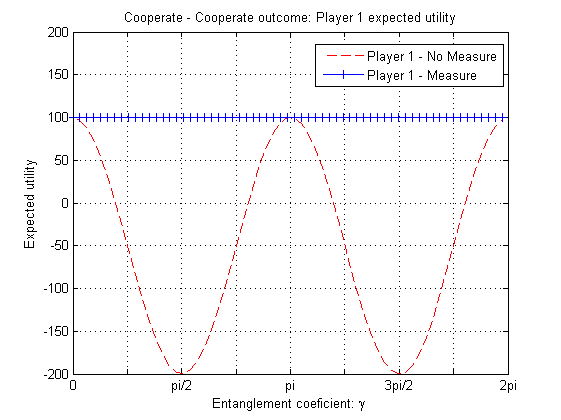
\includegraphics[scale=0.48]{compareluders/CC1.PNG}}
    & b)\putindeepbox[7pt]{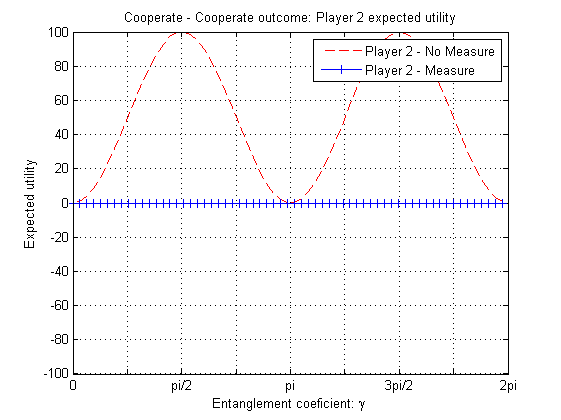
\includegraphics[scale=0.48]{compareluders/CC2.PNG}} \\
  c)\putindeepbox[7pt]{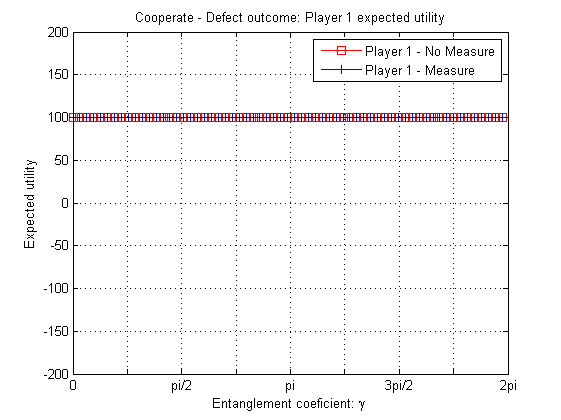
\includegraphics[scale=0.48]{compareluders/CD1.PNG}}
    & d)\putindeepbox[7pt]{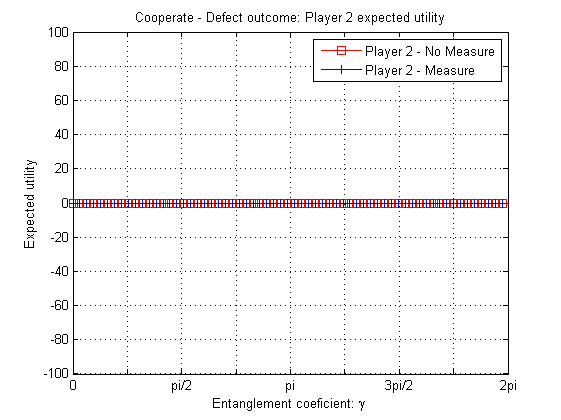
\includegraphics[scale=0.48]{compareluders/CD2.PNG}} \\
  e)\putindeepbox[7pt]{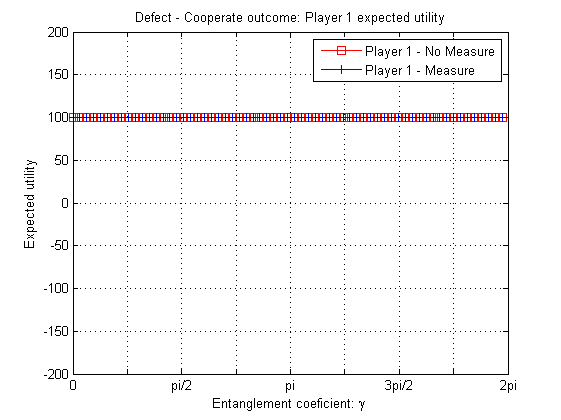
\includegraphics[scale=0.46]{compareluders/DC1.PNG}}
    & f)\putindeepbox[7pt]{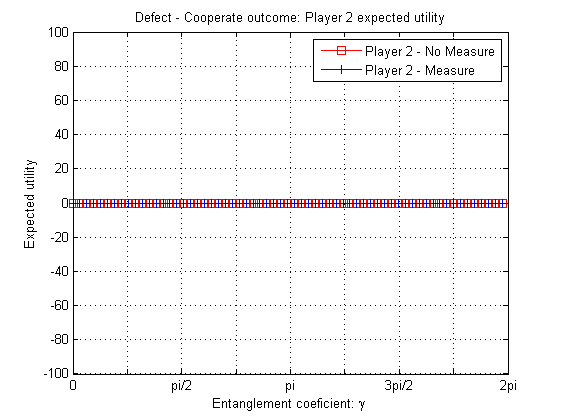
\includegraphics[scale=0.48]{compareluders/DC2.PNG}} \\
  g)\putindeepbox[7pt]{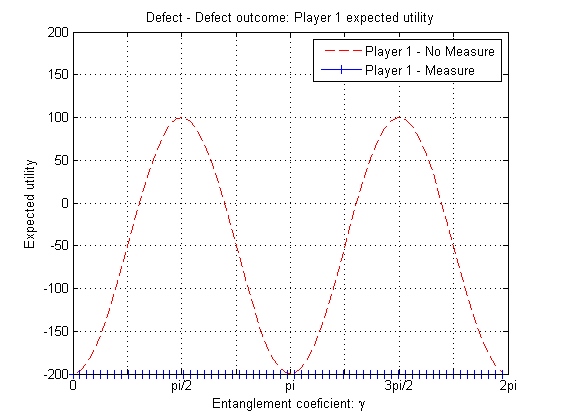
\includegraphics[scale=0.46]{compareluders/DD1.PNG}}
    & h)\putindeepbox[7pt]{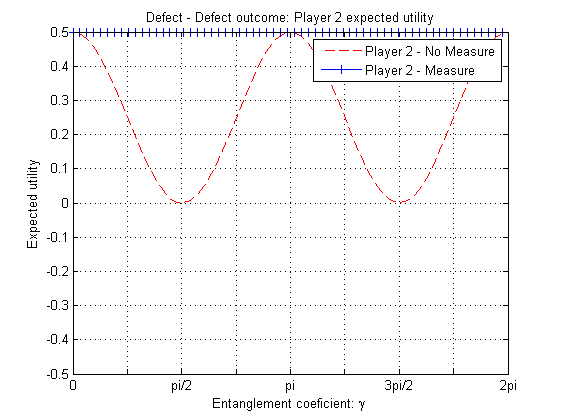
\includegraphics[scale=0.48]{compareluders/DD2.PNG}} \\
\end{tabular}
\caption{Comparison of the expected utilities when measuring and not measuring between steps 1 and 2 of a 3 player game (the player 1 will be the player 2 in the 3 player game, and the player 2 will be the player 3 in the 3 game situation).}
\label{tab:luderscomp}
\end{center}
 \end{table}



We set up a system with $3$ players and in the step $1$ the three players chose the operators $o_{10},o_{21},o_{31}$ producing the outcome $CDD$, the initial proposal for the gold coin division will be $(100, 0, 0)$. 

To analyse the step $2$,  the system will be kept in the initial dimension ($\mathcal{H}^{3}$), because of the following reasons: if we have entangled states, they won't be are separable; There may be various mappings in a lower dimension that fit the higher dimension composition. This means that the previous highest ranking player will no longer have access to the voting operators, instead she will use invariably a symmetric coin operator. 

In one situation we will use the L\"{u}der's Rule, after the voting. This is the equivalent of performing a measurement on the system. In the other situation the two players will act on step $2$. The results for this experiment (Table \ref{tab:luderscomp}), allow us to conclude that not measuring the system affects the expected utilities for the players in two of the four possible analysed outcomes. In this case the act of measuring leaves us with the same utility results one would get in a classic situation with $2$ players game, the equilibrium here is $CD$ outcome. Without the intermediate measuring step the outcome will depend on the $\gamma$ - the initial coefficient used to set up the system. For example:

\begin{itemize}
\item $\gamma = 0$, we have the same results as in the original problem. The Nash equilibrium is unique and it is $CD$.
\item $\gamma = \frac{\pi}{2}$, the equilibrium is $DC$, as the payoffs for the $CC$ outcome are $(-200, 0.5)$, and the outcome $DD$ will present $(100, 0)$ for the expected utilities of the players.
\item $\gamma = \frac{\pi}{4}$, all possible outcomes will be Nash equilibria. As we can see in Table \ref{tab:hate_myself}, no player can improve her payoff by unilaterally changing her strategy.



\end{itemize}

\begin{center}
\begin{table}
\begin{centering}
\begin{tabular}{ccc}
\hline 
 $\gamma = \frac{\pi}{4}$ & Player 2: C & Player 2: D\tabularnewline
\hline 
Player 1: C & (-50, 0.25) & (100, 0)\tabularnewline
Player 1: D & (100, 0) & (-50, 0.25)\tabularnewline
\hline 
\end{tabular}
\par\end{centering}

\caption{Normal form representation of the second step in a 3 player game with an entanglement coefficient of $\frac{\pi}{4}$, where there isn't an intermediate measuring. }
\label{tab:hate_myself}
\end{table}
\end{center}


\subsection{Analysis and Results}
\label{subsec:description_3}


If we measure in between steps where we measure the system in between states, we can fix the payoff functionals for $3$ players in the step 1. In order to do so we will take into account the Nash equilibrium for the $2$ player subgame in \ref{eq:pirates_payoff2} and \label{eq:pirates_payoff3}. The constants $(e_{22}, e_{23})$ will be the pair of utilities for player 2 and 3 in an equilibrium situation, $(e_{22}, e_{23})=(100, 0)$.  
 \begin{equation}
\begin{split}
E_{11}(\vert\psi_{fin1}\rangle, \alpha_{1})=\alpha_{1}\times(\vert\langle000\vert\psi_{fin1}\rangle\vert^{2} + \vert\langle100\vert\psi_{fin1}\rangle\vert^{2}
+ \vert\langle010\vert\psi_{fin1}\rangle\vert^{2}
+ \vert\langle001\vert\psi_{fin1}\rangle\vert^{2}
 ) - \\
 - 200\times(\vert\langle111\vert\psi_{fin1}\rangle\vert^{2} + \vert\langle110\vert\psi_{fin1}\rangle\vert^{2}
+ \vert\langle101\vert\psi_{fin1}\rangle\vert^{2}
+ \vert\langle011\vert\psi_{fin1}\rangle\vert^{2}
 )
\end{split}
\end{equation}

 \begin{equation}
\begin{split}
E_{12}(\vert\psi_{fin1}\rangle, \alpha_{2})=\alpha_{2}\times(\vert\langle000\vert\psi_{fin1}\rangle\vert^{2} + \vert\langle100\vert\psi_{fin1}\rangle\vert^{2}
+ \vert\langle010\vert\psi_{fin1}\rangle\vert^{2}
+ \vert\langle001\vert\psi_{fin1}\rangle\vert^{2}
 ) - \\
 + (0.5 + e_{22})\times(\vert\langle111\vert\psi_{fin1}\rangle\vert^{2} + \vert\langle110\vert\psi_{fin1}\rangle\vert^{2}
+ \vert\langle101\vert\psi_{fin1}\rangle\vert^{2}
+ \vert\langle011\vert\psi_{fin1}\rangle\vert^{2}
 )
\end{split}
\label{eq:pirates_payoff2}
\end{equation}

 \begin{equation}
\begin{split}
E_{13}(\vert\psi_{fin1}\rangle, \alpha_{3})=\alpha_{3}\times(\vert\langle000\vert\psi_{fin1}\rangle\vert^{2} + \vert\langle100\vert\psi_{fin1}\rangle\vert^{2}
+ \vert\langle010\vert\psi_{fin1}\rangle\vert^{2}
+ \vert\langle001\vert\psi_{fin1}\rangle\vert^{2}
 ) - \\
 + (0.5 + e_{23})\times(\vert\langle111\vert\psi_{fin1}\rangle\vert^{2} + \vert\langle110\vert\psi_{fin1}\rangle\vert^{2}
+ \vert\langle101\vert\psi_{fin1}\rangle\vert^{2}
+ \vert\langle011\vert\psi_{fin1}\rangle\vert^{2}
 )
\end{split}
\label{eq:pirates_payoff3}
\end{equation}

\begin{table}

\begin{center}
\begin{tabular}{cc}
  a)\putindeepbox[7pt]{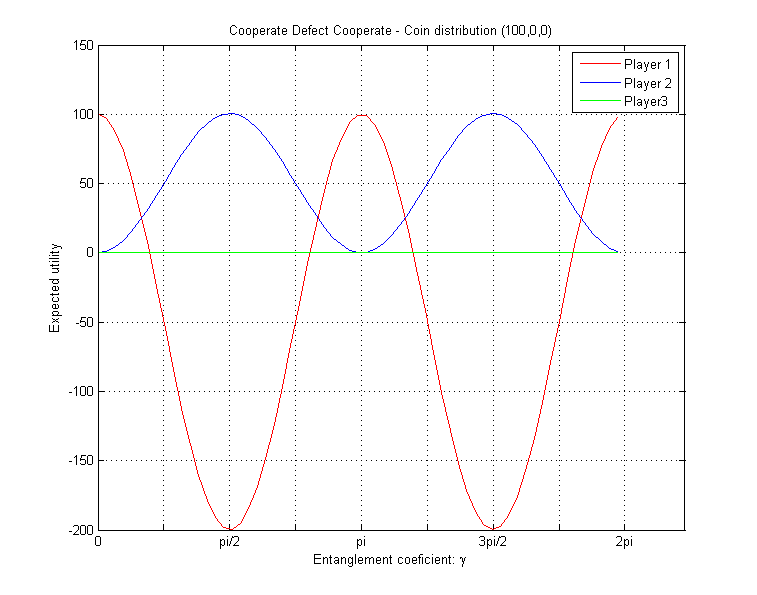
\includegraphics[scale=0.46]{3Players/CDC100_0_0_1.PNG}}
    & a1)\putindeepbox[7pt]{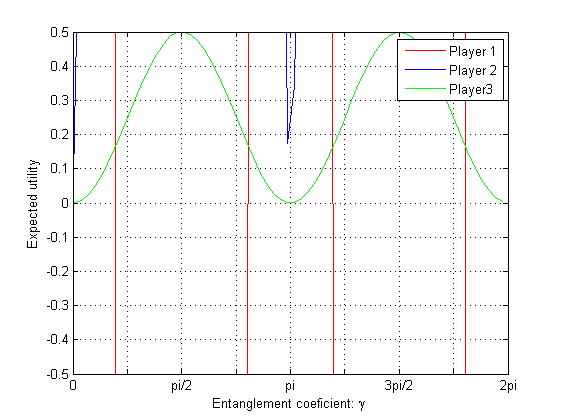
\includegraphics[scale=0.46]{3Players/CDC100_0_0_2.PNG}} \\
\end{tabular}
\caption{Expected utility in a three player situation with intermediate measure step, where the players will use the $(Cooperate, Defect, Cooperate)$ operators. The inicial proposal is $(\alpha_{1}, \alpha_{2}, \alpha_{3}) =(100, 0, 0)$.}
\label{tab:3player}
\end{center}
 \end{table}

\begin{comment}

\begin{table}
\begin{center}
\begin{tabular}{c}
  a)\putindeepbox[7pt]{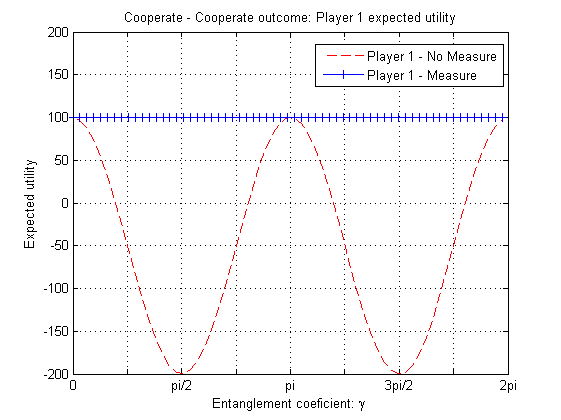
\includegraphics[scale=0.80]{compareluders/CC1.PNG}}\\
  b)\putindeepbox[7pt]{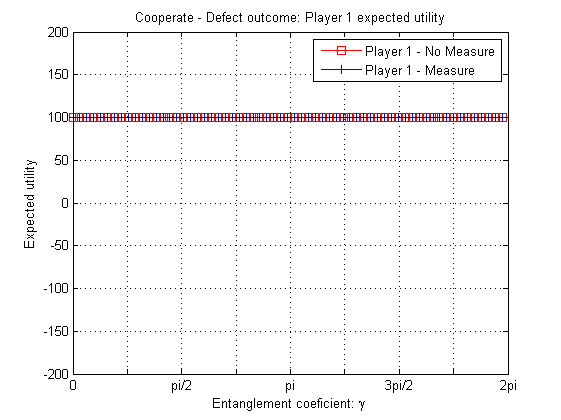
\includegraphics[scale=0.80]{compareluders/CD1.PNG}}\\
  c)\putindeepbox[7pt]{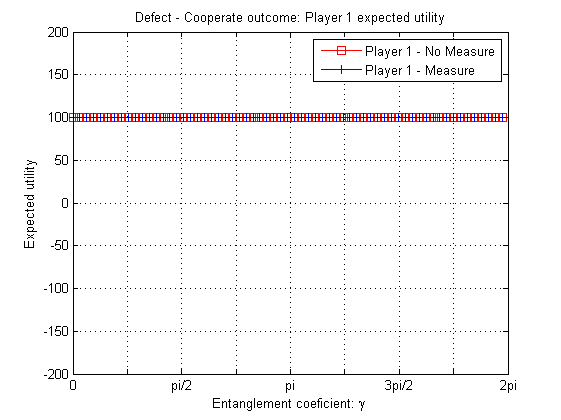
\includegraphics[scale=0.46]{compareluders/DC1.PNG}}\\
  d)\putindeepbox[7pt]{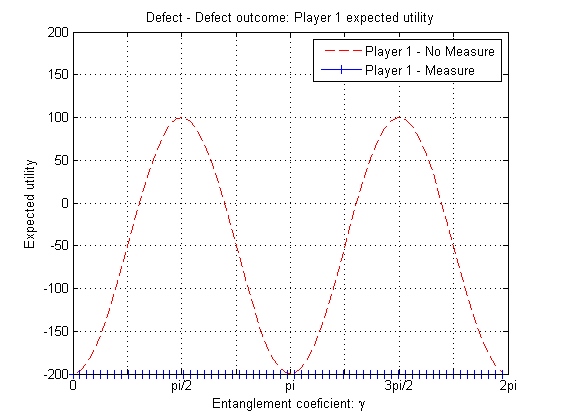
\includegraphics[scale=0.46]{compareluders/DD1.PNG}}\\
\end{tabular}
\caption{Comparison of the expected utilities when measuring and not measuring between steps 1 and 2 of a 3 player game, for the captain (player 2 in the first round). }
\label{tab:luderscomp}
\end{center}
 \end{table}

\begin{table}
\begin{center}
\begin{tabular}{c}
   a)\putindeepbox[7pt]{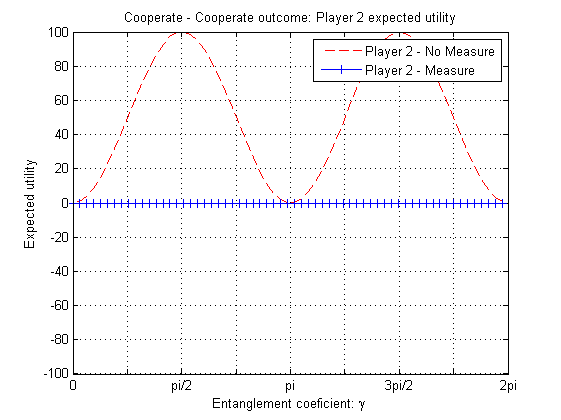
\includegraphics[scale=0.80]{compareluders/CC2.PNG}} \\
   b)\putindeepbox[7pt]{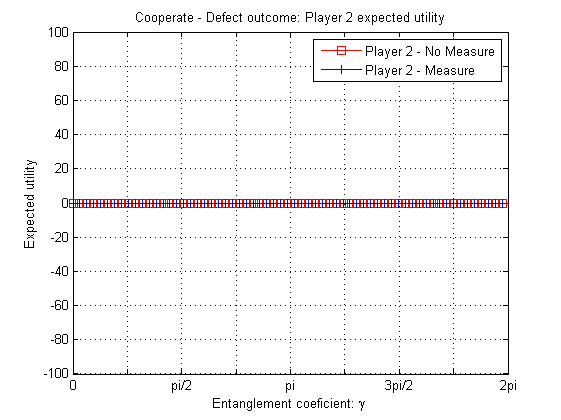
\includegraphics[scale=0.80]{compareluders/CD2.PNG}} \\
   c)\putindeepbox[7pt]{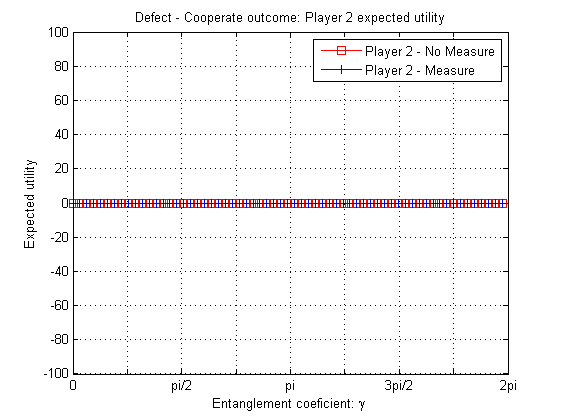
\includegraphics[scale=0.80]{compareluders/DC2.PNG}} \\
   d)\putindeepbox[7pt]{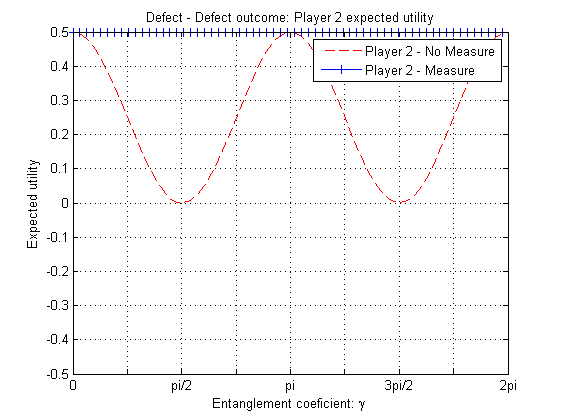
\includegraphics[scale=0.80]{compareluders/DD2.PNG}} \\
\end{tabular}
\caption{Comparison of the expected utilities when measuring and not measuring between steps 1 and 2 of a 3 player game, for the player with the lower ranking (player 3 in the first round). }
\label{tab:luderscomp1}
\end{center}
 \end{table}


''''''Depending on the measurement outcome that occurs with probability x, the players will act on the second round. The L\"{u}der's rule is applied here. The highest ranking player will no longer have access to the voting operators, instead he will only be able to manipulate de system using a symmetric coin operator.

Keeping the system in a higher dimension is considered because of the following reasons: if we have entangled states, they won't be are separable, and there are various mappings to a lower dimension that fit the system composition. 


\begin{emph}
One important aspect is that the payoff functional changes

Initial state: variable to study.
Payoff functions: variable to study.
\end{emph}

\end{comment}